\begin{qitems}

    \begin{bbox}
        \qitem 在带头结点的单链表 $L$ 中,删除所有值为 $x$ 的结点,并释放其空间,假设值为 $x$ 的结点不唯一,请编写算法实现以上操作。
    \end{bbox}

    \begin{bbox}
        \qitem 编写在带头结点的单链表 $L$ 中删除一个最小绝对值的高效算法 (假设该值唯一)。
    \end{bbox}

    \begin{bbox}
        \qitem 编写算法将带头结点的单链表就地逆置,所谓 "就地" 是指辅助空间复杂度为 O(1)。
    \end{bbox}

    \begin{bbox}
        \qitem 设在带头结点的单链表 $L$ 中,所有结点的元素值无序,请编写一个函数,删除表中所有介于给定的两个值 (作为函数参数给出) 之间的元素 (若存在)。
    \end{bbox}

    \begin{bbox}
        \qitem 给定两个单链表,试分析找出两个链表的公共结点的方法 (不用写代码)。
    \end{bbox}

    \begin{bbox}
        \qitem 设 $C = \{a_1, b_1, a_2, b_2, \dots, a_n, b_n\}$ 为线性表,采用带头结点的单链表存放,设计一个就地算法,将其拆分为两个线性表,使得 $A = \{a_1, a_2, \dots, a_n\}, B = \{b_n, \dots, b_2, b_1\}$。
    \end{bbox}

    \begin{bbox}
        \qitem 在一个递增有序的单链表中,存在重复的元素。设计算法删除重复的元素,例如 $(7, 10, 10, 21, 30, 42, 42, 42, 51, 70)$ 将变为 $(7, 10, 21, 30, 42, 51, 70)$。
    \end{bbox}

    \begin{bbox}
        \qitem 设 $A$ 和 $B$ 是两个单链表 (带头结点),其中元素递增有序。设计一个算法从 $A$ 和 $B$ 中的公共元素产生单链表 $C$,要求不破坏 $A, B$ 的结点。
    \end{bbox}

    \begin{bbox}
        \qitem 已知两个集合 $A$ 和 $B$ 分别表示两个集合,其元素递增排列。编制函数,求 $A$ 与 $B$ 的交集,并存放于 $A$ 链表中。
    \end{bbox}

    \begin{bbox}
        \qitem 两个整数序列 $A=a_1, a_2, a_3, \dots, a_m$ 和 $B=b_1, b_2, b_3, \dots, b_n$ 已经存入两个单链表,设计一个算法,判断序列 $B$ 是否是序列 $A$ 的连续子序列?
    \end{bbox}

    \begin{bbox}
        \qitem 设计一个算法用于判断带头结点的循环双链表是否对称。
    \end{bbox}

    \begin{bbox}
        \qitem 有两个循环单链表,链表头指针分别为 $h_1$ 和 $h_2$,编写一个函数将链表 $h_2$ 链接到链表 $h_1$ 之后,
        要求链接后的链表仍保持循环链表形式。
    \end{bbox}

    \begin{bbox}
        \qitem 设有一个带头结点的非循环双链表 $L$, $L$ 中每个结点除有 pre, data 和 next 域外,
        还有一个访问频度域 freq,其值均初始化为零。每当在链表中进行一次 Locate(L, x) 运算时,
        令值为 $x$ 的结点中 freq 域的值增 $1$,并使此链表中的结点保持按访问频度递减的顺序排列,
        且最近访问的结点排在频度相同的结点之前,以便频繁访问的结点总是靠近表头。
        试编写符合上述要求的 Locate(L, x) 函数,返回找到结点的地址,类型为指针。
    \end{bbox}

    \begin{bbox}
        \qitem 设将 $n$ ($n>1$) 个整数存放到不带头结点的单链表 $L$ 中,
        设计算法将 $L$ 中保存的序列循环右移 $P$ ($0<P<n$) 个位置,
        即将 $L$ 中的数据 $(X_0, X_1, \dots, X_{n-1})$ 变换为 $(X_P, X_{P+1}, \dots, X_{n-1}, X_0, X_1, \dots, X_{P-1})$。
        要求:
        \begin{subqitems}
            \subqitem 给出算法的基本设计思想。
            \subqitem 根据设计思想,采用 C 或 C++语言描述算法,关键之处给出注释。
            \subqitem 说明你所设计算法的时间复杂度和空间复杂度。
        \end{subqitems}
    \end{bbox}

    \begin{bbox}
        \qitem 单链表有环,是指单链表的最后一个结点的指针指向链表中的某个结点 (通常单链表的最后一个结点的指针域是空的)。
        试编写算法判断单链表是否存在环。要求:
        \begin{subqitems}
            \subqitem 给出算法的基本设计思想。
            \subqitem 根据设计思想,采用 C 或 C++语言描述算法,关键之处给出注释。
            \subqitem 说明你所设计算法的时间复杂度和空间复杂度。
        \end{subqitems}
    \end{bbox}

    \begin{bbox}
        \qitem 设有一个长度 $n$ ($n$ 为偶数) 的不带头结点的单链表,且结点值都大于 $0$,设计算法求这个单链表的最大孪生和。
        孪生和定义为一个结点值与其孪生结点值之和,对于第 $i$ 个结点 (从 $0$ 开始),其孪生结点为第 $n-i-1$ 个结点。
        要求:
        \begin{subqitems}
            \subqitem 给出算法的基本设计思想。
            \subqitem 根据设计思想,采用 C 或 C++语言描述算法,关键之处给出注释。
            \subqitem 说明你所设计算法的时间复杂度和空间复杂度。
        \end{subqitems}
    \end{bbox}

    \begin{bbox}
        \qitem 【2009 统考真题】已知一个带有表头结点的单链表,结点结构为:
        \begin{center}
        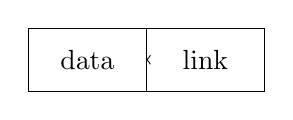
\begin{tikzpicture}
            \node[draw, rectangle, minimum width=1.5cm, minimum height=0.8cm] (data) {data};
            \node[draw, rectangle, minimum width=1.5cm, minimum height=0.8cm, right of=data, node distance=1.5cm] (link) {link};
            \draw[->] (data.east) -- (link.west);
        \end{tikzpicture}
        \end{center}
        假设该链表只给出了头指针 list。在不改变链表的前提下,请设计一个尽可能高效的算法,查找链表中倒数第 $k$ 个位置上的结点 ($k$ 为正整数)。若查找成功,算法输出该结点的 data 域的值,并返回 $1$;否则,只返回 $0$。要求:
        \begin{subqitems}
            \subqitem 描述算法的基本设计思想。
            \subqitem 描述算法的详细实现步骤。
            \subqitem 根据设计思想和实现步骤,采用程序设计语言描述算法 (使用 C、C++或 Java 语言实现),关键之处给出简要注释。
        \end{subqitems}
    \end{bbox}

    \begin{bbox}
        \qitem 【2012 统考真题】假设采用带头结点的单链表保存单词,当两个单词有相同的后缀时,可共享相同的后缀存储空间,例如,loading 和 being 的存储映像如下图所示。
        
        \imgin[0.7]{}{fig/fig2.3.18.png}

        设 str1 和 str2 分别指向两个单词所在单链表的头结点,链表结点结构为 [data] [link],请设计一个时间上尽可能高效的算法,找出由 str1 和 str2 所指向的两个链表共同后缀的起始位置 (如图中字符 i 所在结点的位置 p)。要求:
        \begin{subqitems}
            \subqitem 给出算法的基本设计思想。
            \subqitem 根据设计思想,采用 C 或 C++或 Java 语言描述算法,关键之处给出注释。
            \subqitem 说明你所设计算法的时间复杂度。
        \end{subqitems}
    \end{bbox}

    \begin{bbox}
        \qitem 【2015 统考真题】用单链表保存 $m$ 个整数,结点的结构为 [data] [link],且 |data| $\le n$ ($n$ 为正整数)。现要求设计一个时间复杂度尽可能高效的算法,对于链表中 data 的绝对值相等的结点,仅保留第一次出现的结点而删除其余绝对值相等的结点。例如,若给定的单链表 head 如下:
        
        \imgin[0.7]{}{fig/fig2.3.19.1.png}
        
        则删除结点后的 head 为
        
        \imgin[0.7]{}{fig/fig2.3.19.2.png}
        
        要求:
        \begin{subqitems}
            \subqitem 给出算法的基本设计思想。
            \subqitem 使用 C 或 C++语言,给出单链表结点的数据类型定义。
            \subqitem 根据设计思想,采用 C 或 C++语言描述算法,关键之处给出注释。
            \subqitem 说明你所设计算法的时间复杂度和空间复杂度。
        \end{subqitems}
    \end{bbox}

    \begin{bbox}
        \qitem 【2019 统考真题】设线性表 $L=(a_1,a_2,a_3,\dots,a_{n-2},a_{n-1},a_n)$ 采用带头结点的单链表保存,链表中的结点定义如下:
        \begin{lstlisting}[language=C, basicstyle=\ttfamily\small]
typedef struct node {
    int data;
    struct node*next;
}NODE;
        \end{lstlisting}
        请设计一个空间复杂度为 $O(1)$ 且时间上尽可能高效的算法,重新排列 $L$ 中的各结点,得到线性表 $L'=(a_1,a_n,a_2,a_{n-1},a_3,a_{n-2},\dots)$。要求:
        \begin{subqitems}
            \subqitem 给出算法的基本设计思想。
            \subqitem 根据设计思想,采用 C 或 C++语言描述算法,关键之处给出注释。
            \subqitem 说明你所设计算法的时间复杂度。
        \end{subqitems}
    \end{bbox}

\end{qitems} 